\documentclass[a4paper]{report}

\usepackage[utf8]{inputenc}
\usepackage[T1]{fontenc}
\usepackage[francais]{babel}
\usepackage[colorlinks=true, linkcolor=blue, citecolor=red]{hyperref}
\usepackage{graphicx}
\hypersetup{breaklinks=true}

\title{Les objets connectés}
\author{Bastien \bsc{Labouche}\\Julie \bsc{Lopez}}
\date{24 février 2018}

\begin{document}
	
	\maketitle
	
	\tableofcontents
	
	\newpage
	
	\section{Les objets connectés}
	\subsection{Objets connectés ? Kesako ?}
	Si l'on se base sur la \href{http://objets.insa-rennes.fr/objets-connectes/quest-ce-quun-objet-connecte/}{définition de l'Insa Rennes} :
	\smallbreak
	\begin{quotation}
		un objet connecté est une chose, fabriquée par l’homme, dont l’usage est d’établir une liaison afin de pouvoir faire passer des 					informations diverses et variées à un autre objet ou à toute autre chose connectée.
	\end{quotation}
	\medbreak
	Il s'agit là d'une définition très basique mais assez claire de ce qu'est un objet connecté, même si il n'y a pas vraiment de définition
	"officielle" de ce qu'est un objet connecté. Nous retiendrons donc que ce sont des objets pouvant "communiquer", et ce grâce à différentes
	technologies, par exemple :
	
	\bigbreak
	
	\begin{itemize}
		\item La montre connectée communiquant avec le téléphone grâce au bluetooth.
		\item La caméra IP communiquant via un câble ethernet avec la box.
		\item Le drone piloté avec le téléphone via du wifi.
		\item Le thermostat compatible wifi.
		\item ...
	\end{itemize}

	\bigbreak
	
	Au fur et à mesure de l'avancée de la technologie, une sorte de réseau entre les objets s'est développé, on l'appel "l'internet des objets" 	mais vous le connaissez sûrement sous le nom de IoT (Internet of Things)
	
	\newpage
	
	\subsection{Internet Of Things}
	
	Comme dit plus haut, l'Internet of Things est un réseau reliant entre eux les objets connectés de par le monde, il s'agit de leur version
	d'internet. \href{https://fr.wikipedia.org/wiki/Internet_des_objets}{Selon Wikipedia}, il s'agit d'une extension d'internet qui serait
	considéré comme la troisième évolution de l'internet :
	\smallbreak
	\begin{quotation}
		L'Internet des objets, ou IdO (en anglais Internet of Things, ou IoT), est l'extension d'Internet à des choses et à des lieux du monde
		physique.

		Alors qu'Internet ne se prolonge habituellement pas au-delà du monde électronique, l'Internet des objets connectés représente les
		échanges d'informations et de données provenant de dispositifs du monde réel avec le réseau Internet.
	\end{quotation}
	
	\bigbreak
	
	L'Union internationale des télécommunications nous donne la définition suivante, décrivant l'internet des objets comme une :
	\begin{quotation}
		infrastructure mondiale pour la société de l'information, qui permet de disposer de services évolués en interconnectant 
		des objets(physiques ou virtuels) grâce aux technologies de l'information et de la communication interopérables existantes 
		ou en évolution
	\end{quotation}
	
	\medbreak	
	
	\paragraph{Quelques chiffres}
	\begin{itemize}
		\item En 2016, 5.5 millions d'objets sont connectés chaque jour dans le monde
		\item Gartner inc. prévoit que 26 milliards d'objets seront installés d'ici 2020
		\item Un être humain serait en contact avec 1000 à 5000 objets au cours d'une journée normale
		\item Il ne faut que quelques minutes pour qu'un objet connecté vulnérable se fasse hacker après sa mise en ligne
	\end{itemize}
	
	\newpage	
	
	\section{Failles de sécurité}
	\subsection{Problèmes de configuration}
	Comme vu plus haut dans la partie sur l'IoT des millions (et bientôt des milliards) d'objets sont interconnectés entre eux. Même si
	de nos jours la sécurité des données commence à entrer dans les mœurs, 30\% des objets connectés de l'IoT ne sont toujours pas sécurisés.
	La sécurité est non-seulement négligée du côté des constructeurs, mais aussi du côté des utilisateurs, la plupart ne prenant pas la
	peine de changer les identifiants par défaut, lorsqu'il y en a. Une pratique pouvant facilement être vérifiable en faisant un tour sur 
	Shodan. Il s'agit d'un genre de moteur de recherche pour objets connectés, ce site référence le résultat de balayages de ports massifs
	effectués sur le réseau internet. Cet outil est utilisé par des pirates et chercheurs en sécurité pour trouver des dispositifs mal
	sécurisés et en prendre le contrôle. Le créateur de Shodan a même repéré des failles de sécurité assez importantes comme la possibilité
	de se connecter au système informatique gérant un énorme barrage hydroélectrique en France.
	
	\subsection{Failles systèmes}
	En plus d'être mal configurés, les objets connectés embarquent avec eux de nombreuses failles. En effet, ils sont développés avec
	une idée de praticité, ils sont fait pour être facilement utilisables. Les concepteurs ne les conçoivent pas en pensant à les rendre
	sécurisés. En effet, l'internet des objets est semblable aux débuts de l'internet actuel :
	\medbreak
	\begin{itemize}
		\item Pas de cryptage des données.
		\item Faible conscience des vulnérabilités et possibles attaques.
		\item ...
	\end{itemize}
	\smallbreak
	Même sur d'importants systèmes il peut y avoir des failles extrêmement grave, 
	\href{https://www.objetconnecte.com/les-objets-connectes-un-risque-de-cybersecurite-majeur-dans-lentreprise-2310/}{par exemple}, 
	le 17 avril 2015 un chercheur en sécurité nommé Chris Roberts s'est fait arrêter par le FBI car il a piraté en plein vol l'avion
	de ligne dans lequel il se trouvait. Se permettant en passant de modifier légèrement la trajectoire de l'avion (sans qu'il y ait
	de conséquences pour les passagers). Comment il a fait ? Il a ouvert le boîtier situé sous chaque siège et y a relié son ordinateur via
	un câble ethernet, obtenant ainsi un accès au système d'information de l'appareil.\\
	
	Par exemple, on peut parler des toilettes Statis distribuées par la firme LIXIL Corporation. Il s'agit de toilettes "intelligentes" contrôlées par une application Android se connectant au toilette en établissant une connexion bluetooth. Le problème ? La toilette a un PIN bluetooth de "0000" codé en brut.
	\begin{verbatim}
	BluetoothDevice localBluetoothDevice = 
	BluetoothManager.getInstance().execPairing(paramString, "0000")
	\end{verbatim}
	Ce qui fait que quelqu'un ayant l'application peut contrôler n'importe quel toilette si celle-ci est en mode d'appairage. Sinon il est toujours possible de s'appairer avec le toilette en analysant le trafic bluetooth, trouver son adresse matériel pour ensuite procédé à l'appairage.
	
	\begin{center}
		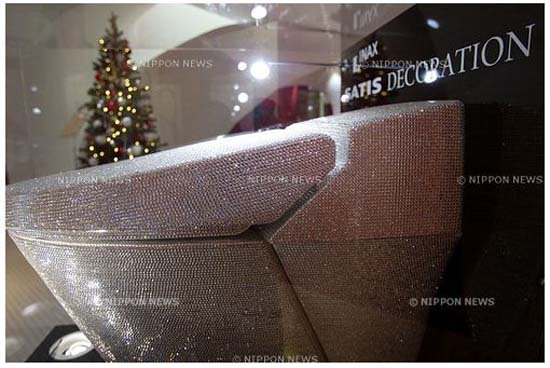
\includegraphics[scale=0.75]{Images/statisToilet.jpg}
		Toilettes Statis
	\end{center}
	
	\newpage
	
	\section{Pourquoi c'est dangereux}
	\subsection{BotNet}
	
	\bigbreak	
	
	\begin{flushleft}
		\textbf{Qu'est-ce qu'un BotNet ?} \\
	\end{flushleft}
	
	Avant de commencer à parler de la menace des BotNet, il est essentiel de définir ce qu'est un botnet.
	BotNet, ce nom est formé de "bot" pour robot et "net" pour network (réseau en français), il désignait à l'origine les réseaux de robots
	IRC mais le terme s'est élargis aux réseaux de machines zombies.
	
	\bigbreak
	
	À l'origine bienveillants, les botnets servaient à proposer divers services aux usagers de IRC, cependant, leur nature première a été 
	détournée à des fins malveillantes. Ces botnets malveillants servent aujourd'hui principalement à :
	\begin{itemize}
		\item Identifier et infecter d’autres machines par diffusion de virus et de programmes malveillants (malwares).
		\item Participer à des attaques groupées de déni de service (DDoS).
		\item Relayer du spam pour du commerce illégal ou pour de la manipulation d'information (par exemple des cours de bourse).
		\item Réaliser des opérations d'hameçonnage.
		\item Générer de façon abusive des clics sur un lien publicitaire au sein d’une page web (fraude au clic).
		\item Exploiter la puissance de calcul des machines ou effectuer des opérations de calcul distribué notamment pour cassage de mots 
		de passe
		\item Mener des opérations de commerce illicite en gérant l'accès à des sites de ventes de produits interdits ou de contrefaçons 
		via des techniques de fast flux, simple ou double-flux ou RockPhish.
		\item Miner des BitCoins
	\end{itemize}
	\href{https://fr.wikipedia.org/wiki/Botnet#Usages_des_botnets}{Source.}
	\bigbreak
		
	Comme vous vous en doutez avec tout ce qui a été dit sur les failles de sécurité, il doit être relativement aisé pour un pirate
	de se constituer un réseau de botnet grâce aux objets connectés, c'est le cas du fameux botnet "Mirai", ce botnet cible les objets
	connectés.
	
	\bigbreak
	
	\begin{flushleft}
		\textbf{Fonctionnement du botnet Mirai} \\
	\end{flushleft}
	
	\textbf{Première étape, reconnaissance :} Le botnet se propage de machine infectée en machine infectée. Une machine infectée 
	va tout d'abord générer une adresse IP aléatoire et la soumettre à une liste noire, si elle ne figure pas dans la liste, 
	la machine zombie va essayer de s'y connecter en essayant divers couples d'identifiants par défaut des constructeurs. On y retrouve 
	essentiellement des caméras, mais aussi des imprimantes, routeurs ou téléphones de VoIP.
	
	\medbreak

	\textbf{Deuxième étape, signalement des victimes potentielles :} Une fois que la machine zombie a pu se connecter grâce à un couple
	identifiant/mot de passe, elle renvoie toutes les informations relative à la victime à un serveur de rapports.
	
	\medbreak
	
	\textbf{Troisième étape, infection :} L'assaillant peut à ce moment là, s'il le désire, se connecter au serveur de rapports et choisir
	ou non d'infecter la nouvelle victime. S'il choisit de le faire, une image
	BusyBox\footnote{Logiciel qui implémente un grand nombre de commandes standard sous Unix.} malveillante est envoyée sur la victime. \\
	La victime fait désormais partie du botnet et commence lui aussi à chercher de nouvelles victimes.
	
	\medbreak
	A partir de ce réseau, le pirate peut lancer toutes sortes d'attaques, comme des attaques de dénis de service ou de ACK flood.
	
	\subsection{Souriez, vous êtes filmés}
	Les objets connectés sont partout, dans les entreprises comme dans les lieux privés, on pense tous qu'ils nous facilitent la vie, et c'est vrai. On peut garder un œil sur sa propre maison ou sur les employés, on peut contrôler la température du frigo ou celle de la salle des serveurs. Ce que l'on ne sait pas c'est que toutes ces nouvelles fonctionnalités ne sont pas protégées.\\ 
	
	On veut créer plus de technologies de plus en vite, avec peu de moyens et on laisse donc de côté la sécurité, mais ce que l'on oublie facilement c'est que ces objets connectés ont accès à des données personnelles (souvent) sensibles. Donc, en ne prenant pas en compte cette sécurité, on laisse libre cours aux hackers ou autres l'accès à ces données sensibles. \\ 
	
	Ce qui fait que n'importe qui peut avoir accès à la petite caméra de surveillance super chouette que l'on a placée dans le salon de notre maison et que tout le monde peut nous "surveiller". N'importe qui peut donc utiliser par exemple Shodan pour trouver tous les objets connectés (et surtout mettre en avant ceux qui ne sont pas sécurisés) et se connecter à la caméra et constater qu'à certains moments les locataires/propriétaires ne sont pas là, et donc programmer un petit cambriolage.\\ 

	Deux journalistes du Rue89 ont même réussi, en utilisant Shodan, à se connecter en quelques clics, à une imprimante à distance, ou encore à la webcam d'un ordinateur particulier. Ils ont pu ainsi, faire une impression à distance sur une imprimante d'un laboratoire de recherche, ce qui a dû leur causer une sacrée surprise.
	Ils auraient même pu, s'ils le voulaient changer la température d'un climatiseur ou encore contrôler la porte d'un garage. Cela peut donc se révéler très dangereux. 	
	
	
	\section{Conclusion}
	
	Les objets connectés, ces petits appareils ont révolutionnés le WEB tout en lançant le phénomène Big Data. Au moment où j'écris ces
	lignes ils sont des milliards à être connectés sur l'IoT. Cependant, même si ils nous facilitent la vie au quotidien, ces objets
	représentent à l'heure actuelle une menace pour la sécurité de nos données et peuvent mettre des vies en danger. En effet, comme cela
	a été évoqué plus haut, un chercheur en sécurité a réussis à détourner un avion sans même avoir eu à se lever de son siège passager. On
	retrouve également des appareils de santé connectés à l'IoT. Malgré tout ceci, les constructeurs n'ont toujours pas à cœur de sécuriser
	leurs produits, et nombre d'entre eux sont mis en ligne sans que leurs propriétaires n'en changent les mots de passe par défauts.\\
	En résumé, les objets connectés sont une révolution, mais il est impératif de les sécuriser sous peine de créer une faille dans son système
	ou de voir ses données dérobées, dans le meilleur des cas.
	
	\subsection{Conseils d'amélioration}
	Les objets connectés, si utiles mais tellement vulnérables... Voici quelques conseils pour sécuriser tout ça :
	\begin{itemize}
		\item Donner la possibilité à l'utilisateur de changer les mots de passe par défauts et insister pour qu'il le fasse.
		\item Si création d'un réseau wifi ne pas permettre à n'importe qui de s'y connecter (mots de passes !).
		\item Chiffrer les donnés échangées.
		\item Chiffrer les données stockées.
		\item Sécuriser les interfaces lorsqu'il y en a.
	\end{itemize}
	
	\newpage
	\section{Sources}
	\begin{itemize}
		\item \href{https://www.digital.security/en/blog/threats-connected-objects-issues-and-possibilities}{Digital Security}
		
		\item \href{https://www.objetconnecte.com/les-objets-connectes-un-risque-de-cybersecurite-majeur-dans-lentreprise-2310/}{objetconnecte.com}
		
		\item \href{https://www.objetconnecte.com/fbi-securite-iot-2409/}{objetconnecte.com}
		\item \href{https://fr.wikipedia.org/wiki/Shodan_%28site_web%29}{Wikipedia}
		\item \href{https://www.francetvinfo.fr/replay-radio/hyper-revue-de-presse/shodan-le-moteur-de-recherche-qui-se-connecte-a-votre-insu_1762849.html}{Francetvinfo}
		\item \href{http://objets.insa-rennes.fr/objets-connectes/quest-ce-quun-objet-connecte/}{Insa-rennes}
		\item \href{https://fr.wikipedia.org/wiki/Internet_des_objets}{Wikipedia}
		\item \href{https://fr.wikipedia.org/wiki/Botnet#Usages_des_botets}{Wikipedia}
		\item \href{https://www.sentryo.net/fr/botnet-iot-mirai-menace-cle-en-main-rendue-publique/}{sentryo.net}
	\end{itemize}
	
\end{document}
